\documentclass{article}

\usepackage{amsmath, amsthm, amssymb, amsfonts}
\usepackage{thmtools}
\usepackage{graphicx}
\usepackage{setspace}
\usepackage{geometry}
\usepackage{float}
\usepackage{hyperref}
\usepackage[utf8]{inputenc}
\usepackage[english]{babel}
\usepackage{framed}
\usepackage[dvipsnames]{xcolor}
\usepackage{tcolorbox}

\colorlet{LightGray}{White!90!Periwinkle}
\colorlet{LightOrange}{Orange!15}
\colorlet{LightGreen}{Green!15}
\colorlet{LightBlue}{Blue!15}

\newcommand{\HRule}[1]{\rule{\linewidth}{#1}}

\declaretheoremstyle[name=Theorem,]{thmsty}
\declaretheorem[style=thmsty,numberwithin=section]{theorem}
\tcolorboxenvironment{theorem}{colback=LightGray}

\declaretheoremstyle[name=Proposition,]{prosty}
\declaretheorem[style=prosty,numberlike=theorem]{proposition}
\tcolorboxenvironment{proposition}{colback=LightOrange}

\declaretheoremstyle[name=Definition,]{prcpsty}
\declaretheorem[style=prcpsty,numberlike=theorem]{definition}
\tcolorboxenvironment{definition}{colback=LightGreen}

\declaretheoremstyle[name=Remark,]{prosty}
\declaretheorem[style=prosty,numberlike=theorem]{remark}
\tcolorboxenvironment{remark}{colback=LightBlue}

\setstretch{1.2}
\geometry{
    textheight=9in,
    textwidth=5.5in,
    top=1in,
    headheight=12pt,
    headsep=25pt,
    footskip=30pt
}

% ------------------------------------------------------------------------------

\begin{document}

% ------------------------------------------------------------------------------
% Cover Page and ToC
% ------------------------------------------------------------------------------

\title{ \normalsize \textsc{}
		\\ [2.0cm]
		\HRule{1.5pt} \\
		\LARGE \textbf{\uppercase{MATH 510 Basics}
		\HRule{2.0pt} \\ [0.6cm] \LARGE{Speedin' Algebraic Geometry 1} \vspace*{10\baselineskip}}
		}
\date{}
\author{\textbf{Rafael Barroso} \\ 
		Mathematics Ing. \\
		EPFL \\
		\today}

\maketitle
\newpage

\tableofcontents
\newpage

% ------------------------------------------------------------------------------

\section{Algebraic definitions} \label{sec:alg-def}
We first explore some algebraic definitions in order to fully grasp the language Algebraic Geometry is spoken in; commutative algebra.
As a personal view, algebra is about exploring how mathematical objects are combined with others in order to produce much more sensual ones via operations, hence we start by defining that which is most basic.

\vspace{0.3cm}

\begin{definition}
    A \textit{group} $\mathcal{G}$ is a set $S$ together with a \textit{binary operation} $\otimes$ such that the following rules are met.
    \begin{itemize}
        \item \textbf{Associativity : } $\forall$ $a,b,c \text{ } \in S$ we have $a \otimes (b \otimes c) = (a \otimes b) \otimes c$.
        \item \textbf{Identity :} $\exists \text{ } e_S \in S \text{ } : \text{ } a \otimes e_S = e_S \otimes a = a$.
        \item \textbf{Inverse : } $\forall \text{ } a \in S \text{ } \exists \text{ } a^{-1} \in S \text{ } : \text{ } a \otimes a^{-1} = a^{-1} \otimes a = e_S$.
    \end{itemize} 
\end{definition}

\vspace{0.3cm}

A binary operarion is a \textit{function} that combines two elements from a single set and produces annother element from the same set. This property is sometimes considered as one of the "rules" (i.e. \textit{Closure}) required
in order to form a group $\mathcal{G}$.

\vspace{0.3cm}

\begin{remark}
    Note that it is not necesary that the following "rule" is met in order to costruct a group. \textbf{Commutativity :} $\forall a,b \in \mathcal{G} \text{ : } a \otimes b = b \otimes a$. Whenever our group in question
    meeets this requirement, we call it an \textit{abelian} group.
\end{remark}

\vspace{0.3cm}

We now explore what happens whenever we throw annother operation into the mix. It is customary (as for all the books I've read) that the operations being considered are \textit{addition} commonly denoted as
$+$ and \textit{multiplication}. For personal reasons (mainly lazyness), we denote the product of $a,b \in \mathcal{G}$ as $ab$.

\vspace{0.3cm}

\begin{definition}

    A \textit{ring} $\mathcal{R}$ is a set, together with two binary operations (i.g. addition and multiplication) such that:

    \begin{itemize}
        \item $\mathcal{R}$ is an abelian group with respect to addition (it has a neutral element denoted by 0, and $\forall \text{ } x \in \mathcal{R} \text{  } \exists \text{  } x^{-1}=-x \text{ }: \text{ } x+(-x)=0 $).
        \item Multiplication is associative $x(yz)=(xy)z$ and distributive over addition $x(y+z)=xy+xz, \text{  } (x+y)z=xz+yz$.
    \end{itemize}

\end{definition}

\vspace{0.3cm}

One can also make $\mathcal{R}$ an abelian group with respect to multiplication, hence making it an ever sexier algebraic structure. We present a cool figure \ref{fig:flav-ring}
with all of the flavors a ring may get from adding certain 'rules' into our group with respect to our secondary operation.

\vspace{0.3cm}
    
\begin{remark} 
    Of course, we do not exclude the possibility that $1=0$, thus we have: $$\forall \text{ } x \in \mathcal{R}:x1=x0=0 \implies \mathcal{R} = 0$$
    the \textbf{zero} ring.
\end{remark}

\vspace{0.3cm}

A \textit{commutative ring} is a ring $\mathcal{R}$ where the secondary operation is commutative. We also have rings with \textit{unity}, often called \textit{ring with identity}; all 
fancy wording for stating that the ring has an identity element with respect to its secondary operation. Combining these two flvors and creating a new 'rule', we get a special type of ring called 
\textit{integral domains}. If we only have a ring with identity and generate an inverse element for all elements with respect to the secondary operation, we get a \textit{division ring}.

\vspace{0.3cm}

\begin{definition}
    An integral domain is a commutative ring with unity $\mathcal{I}$ such that $\forall a,b \in \mathcal{I} \text{ : } ab = 0 \implies a = 0 \text{ or } b = 0$.    
\end{definition}

\vspace{0.3cm}

Finally, adding all of these properties onto our definition $1.3$ makes the most delicious algebraic structure (personal pov); a \textit{field}.

\begin{figure}[h!] % 'h!' for positioning
    \centering
    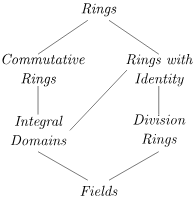
\includegraphics[scale=0.5]{figures/ring_flavors.png} % scale the figure here
    \caption{Ring flavors \cite{judson2019abstract}.}
    \label{fig:flav-ring}
\end{figure}

In order to understand if these types of objects are 'the same', we buld mappings element-wise (i.e. functions) and check if certain properties are met.
There are two main types of mappings that tell us whenever two things have the same structure, these are \textit{homomorphisms} and \textit{isomorphisms} where the latter implies stronger equality.

\vspace{0.3cm}

\begin{definition}
    A \textit{ring homomorphism} is a mapping $g \text{ : }  \mathcal{A} \rightarrow \mathcal{B}$ such that: 
    \begin{itemize}
        \item $g(a+b) = g(a) + g(b) \text{ } \forall a,b \in \mathcal{A}$
        \item $g(ab) = g(a) g(b) \text{ } \forall a,b \in \mathcal{A}$
        \item $g(e^+_{\mathcal{A}}) = e^+_{\mathcal{B}}$
    \end{itemize}
    where $\mathcal{A}, \mathcal{B}$ are rings and $e^+_{\mathcal{A}}, e^+_{\mathcal{A}}$ are the additive identies respectively.
\end{definition}

\newpage

This means that both rings are \textit{roughly} the same. In order to state their full 'masked equality' (i.e. same structure, diferent costume), we define the following notion.

\vspace{0.3cm}

\begin{definition}
    A \textit{ring isomorphism} is a \textit{$1-1$ mapping} $\phi \text{ : } \mathcal{A} \rightarrow \mathcal{B}$ which is also a ting homomorphism.
\end{definition}

\vspace{0.3cm}

Whenever we say that a function is a $1-1$ mapping we mean a \textit{bijective} function. Note that the definitions of \textit{group homomorphism} and \textit{group isomorphism} are the same as for rings
but we just omit the secondary operation.

\vspace{0.3cm}

\begin{remark}
    Whenever our two rings; $\mathcal{A}, \mathcal{B}$, are rings have a secondary identity, it must be that $\psi(e^{\cdot}_{\mathcal{A}}) = e^{\cdot}_{\mathcal{B}}$ in order for $\psi: \mathcal{A} \rightarrow \mathcal{B}$ to be a ring homomorphism.
\end{remark}

\newpage

\section{Examples} \label{sec:examples}
% ----------------------- EXAMPLES OF USAGE ------------------------
\begin{theorem}
    This is a theorem.
\end{theorem}

\begin{proposition}
    This is a proposition.
\end{proposition}

\begin{definition}
    This is a principle.
\end{definition}

This is a citation to a great book \cite{atiyah1969introduction}.
% ------------------------------------------------------------------

\newpage

% ------------------------------------------------------------------------------
% Reference and Cited Works
% ------------------------------------------------------------------------------

\bibliographystyle{IEEEtran}
\bibliography{biblio.bib}

% ------------------------------------------------------------------------------

\end{document}
